\documentclass[aspectratio=43]{beamer}
% \documentclass[aspectratio=169]{beamer}

% Title --------------------------------------------
\title[Lecture 4: Causal methods]{\Large Causal methods with observational data}
\author[]{Francisco Villamil}
\date[]{Research Design for Social Sciences\\MA Computational Social Science, UC3M\\Fall 2023}

%%% NOTE -- CHECK THIS: https://github.com/paulgp/beamer-tips


%%% Building heavily on https://github.com/kylebutts/templates

% xcolor, define them
\usepackage{xcolor}

% TEXT COLORS
\definecolor{red}{HTML}{9a2515}
\definecolor{yellow}{HTML}{EBC944}
\definecolor{asher}{HTML}{555F61}
\definecolor{jet}{HTML}{131516}

% THEME COLORS
\definecolor{accent}{HTML}{107895}
\definecolor{accent2}{HTML}{9a2515}

% Color commands
\newcommand\red[1]{{\color{red}#1}}
\newcommand\yellow[1]{{\color{yellow}#1}}
\newcommand\asher[1]{{\color{asher}#1}}

\newcommand\BGred[1]{{\colorbox{red!80!white}{#1}}}
\newcommand\BGyellow[1]{{\colorbox{yellow!80!white}{#1}}}
\newcommand\BGasher[1]{{\colorbox{asher!80!white}{#1}}}

% Appendix numbering
\usepackage{appendixnumberbeamer}

% Beamer Options -------------------------------------

% Background
\setbeamercolor{background canvas}{bg = white}

% Change text margins
\setbeamersize{text margin left = 25pt, text margin right = 15pt}

% \alert
\setbeamercolor{alerted text}{fg = accent2}

% Frame title
\setbeamercolor{frametitle}{bg = white, fg = jet}
\setbeamercolor{framesubtitle}{bg = white, fg = accent}
\setbeamerfont{framesubtitle}{size = \small, shape = \itshape}

% Block
\setbeamercolor{block title}{fg = white, bg = accent2}
\setbeamercolor{block body}{fg = jet, bg = jet!10!white}

% Title page
\setbeamercolor{title}{fg = jet}
\setbeamercolor{subtitle}{fg = accent}

%% Custom \maketitle and \titlepage
\setbeamertemplate{title page}
{
    \begin{centering}
      % \vspace{20mm}
      {\Large \usebeamerfont{title}\usebeamercolor[fg]{title}\inserttitle}\\ \vskip0.25em%
      \ifx\insertsubtitle\@empty%
      \else%
        {\usebeamerfont{subtitle}\usebeamercolor[fg]{subtitle}\insertsubtitle\par}%
      \fi%
      {\vspace{10mm}\insertauthor}\\
      \ifx\insertinstitute\@empty%
      \else%
        {\vspace{5mm}\color{asher}\scriptsize{\insertinstitute}}\\\vspace{5mm}
      \fi%
      {\color{asher}\small{\insertdate}}\\
    \end{centering}
}

% Table of Contents
\setbeamercolor{section in toc}{fg = accent!70!jet}
\setbeamercolor{subsection in toc}{fg = jet}

% Button
\setbeamercolor{button}{bg = accent}

% Remove navigation symbols
\setbeamertemplate{navigation symbols}{}

% Table and Figure captions
\setbeamercolor{caption}{fg=jet!70!white}
\setbeamercolor{caption name}{fg=jet}
\setbeamerfont{caption name}{shape = \itshape}

% Put slide number / total slides at the bottom right
\makeatother
\makeatletter
\setbeamertemplate{footline} %{\hfill\insertframenumber/\inserttotalframenumber}
{%
  \leavevmode%
  \hbox{
  \begin{beamercolorbox}[wd=\paperwidth,ht=2.5ex,dp=1.125ex,leftskip=.3cm,rightskip=.3cm plus1fil]{footlinecolor}%
    \color{asher}{{\let\hyperlink\@secondoftwo\insertshorttitle}\hfill\insertshortauthor\hfill\insertshortdate\hfill\insertframenumber/\inserttotalframenumber}
  \end{beamercolorbox}}%
  \vskip0pt%
}
\makeatother
\makeatletter

% Bullet points

%% Fix left-margins
\settowidth{\leftmargini}{\usebeamertemplate{itemize item}}
\addtolength{\leftmargini}{\labelsep}

%% enumerate item color
\setbeamercolor{enumerate item}{fg = accent}
\setbeamerfont{enumerate item}{size = \small}
\setbeamertemplate{enumerate item}{\insertenumlabel.}

%% itemize
\setbeamercolor{itemize item}{fg = accent!70!white}
\setbeamerfont{itemize item}{size = \small}
\setbeamertemplate{itemize item}[circle]
\setlength{\itemsep}{0pt plus 6pt}

%% right arrow for subitems
\setbeamercolor{itemize subitem}{fg = accent!60!white}
\setbeamerfont{itemize subitem}{size = \small}
\setbeamertemplate{itemize subitem}{$\rightarrow$}

\setbeamertemplate{itemize subsubitem}[square]
\setbeamercolor{itemize subsubitem}{fg = jet}
\setbeamerfont{itemize subsubitem}{size = \small}

% References

%% Bibliography Font, roughly matching aea
\setbeamerfont{bibliography item}{size = \footnotesize}
\setbeamerfont{bibliography entry author}{size = \footnotesize, series = \bfseries}
\setbeamerfont{bibliography entry title}{size = \footnotesize}
\setbeamerfont{bibliography entry location}{size = \footnotesize, shape = \itshape}
\setbeamerfont{bibliography entry note}{size = \footnotesize}

\setbeamercolor{bibliography item}{fg = jet}
\setbeamercolor{bibliography entry author}{fg = accent!60!jet}
\setbeamercolor{bibliography entry title}{fg = jet}
\setbeamercolor{bibliography entry location}{fg = jet}
\setbeamercolor{bibliography entry note}{fg = jet}

%% Remove bibliography symbol in slides
\setbeamertemplate{bibliography item}{}





% Links ----------------------------------------------

\usepackage{hyperref}
\hypersetup{
  colorlinks = true,
  linkcolor = accent2,
  filecolor = accent2,
  urlcolor = accent2,
  citecolor = accent2,
}


% Line spacing --------------------------------------
\usepackage{setspace}
\setstretch{1.2}


% \begin{columns} -----------------------------------
\usepackage{multicol}


% % Fonts ---------------------------------------------
% % Beamer Option to use custom fonts
% \usefonttheme{professionalfonts}
%
% % \usepackage[utopia, smallerops, varg]{newtxmath}
% % \usepackage{utopia}
% \usepackage[sfdefault,light]{roboto}
%
% % Small adjustments to text kerning
% \usepackage{microtype}



% Remove annoying over-full box warnings -----------
\vfuzz2pt
\hfuzz2pt


% Table of Contents with Sections
\setbeamerfont{myTOC}{series=\bfseries, size=\Large}
\AtBeginSection[]{
        \frame{
            \frametitle{Roadmap}
            \tableofcontents[current]
        }
    }


% References ----------------------------------------
\usepackage[
    citestyle= authoryear,
    style = authoryear,
    natbib = true,
    backend = biber
]{biblatex}

% Smaller font-size for references
\renewcommand*{\bibfont}{\small}

% Remove "In:"
\renewbibmacro{in:}{}

% Color citations for slides
\newenvironment{citecolor}
    {\footnotesize\begin{color}{accent2}}
    {\end{color}}

\newcommand{\citetcolor}[1]{{\footnotesize\textcolor{asher}{\citet{#1}}}}
\newcommand{\citepcolor}[1]{{\footnotesize\textcolor{asher}{\citep{#1}}}}

% Tables -------------------------------------------
% Tables too big
% \begin{adjustbox}{width = 1.2\textwidth, center}
\usepackage{adjustbox}
\usepackage{array}
\usepackage{threeparttable, booktabs, adjustbox}

% Fix \input with tables
% \input fails when \\ is at end of external .tex file

\makeatletter
\let\input\@@input
\makeatother

% Tables too narrow
% \begin{tabularx}{\linewidth}{cols}
% col-types: X - center, L - left, R -right
% Relative scale: >{\hsize=.8\hsize}X/L/R
\usepackage{tabularx}
\newcolumntype{L}{>{\raggedright\arraybackslash}X}
\newcolumntype{R}{>{\raggedleft\arraybackslash}X}
\newcolumntype{C}{>{\centering\arraybackslash}X}

% Figures

% \imageframe{img_name} -----------------------------
% from https://github.com/mattjetwell/cousteau
\newcommand{\imageframe}[1]{%
    \begin{frame}[plain]
        \begin{tikzpicture}[remember picture, overlay]
            \node[at = (current page.center), xshift = 0cm] (cover) {%
                \includegraphics[keepaspectratio, width=\paperwidth, height=\paperheight]{#1}
            };
        \end{tikzpicture}
    \end{frame}%
}

% subfigures
\usepackage{subfigure}


% Highlight slide -----------------------------------
% \begin{transitionframe} Text \end{transitionframe}
% from paulgp's beamer tips
\newenvironment{transitionframe}{
    \setbeamercolor{background canvas}{bg=accent!60!black}
    \begin{frame}\color{accent!10!white}\LARGE\centering
}{
    \end{frame}
}


% Table Highlighting --------------------------------
% Create top-left and bottom-right markets in tabular cells with a unique matching id and these commands will outline those cells
\usepackage[beamer,customcolors]{hf-tikz}
\usetikzlibrary{calc}
\usetikzlibrary{fit,shapes.misc}

% To set the hypothesis highlighting boxes red.
\newcommand\marktopleft[1]{%
    \tikz[overlay,remember picture]
        \node (marker-#1-a) at (0,1.5ex) {};%
}
\newcommand\markbottomright[1]{%
    \tikz[overlay,remember picture]
        \node (marker-#1-b) at (0,0) {};%
    \tikz[accent!80!jet, ultra thick, overlay, remember picture, inner sep=4pt]
        \node[draw, rectangle, fit=(marker-#1-a.center) (marker-#1-b.center)] {};%
}


\usepackage{amsmath}
\renewcommand<>{\BGyellow}[1]{\only#2{\beameroriginal{\BGyellow}}{#1}}

\begin{document}
% ====================================================

% ----------------------------------------------------
\begin{frame}
  \titlepage
\end{frame}
% ----------------------------------------------------

\section{Intro and overview}

% ----------------------------------------------------
\begin{frame}
\frametitle{Re-cap}
\centering

\begin{itemize}
  \item[1.] Problem/topic
  \item[2.] Stories, arguments about mechanisms
  \item[3.] Research question
  \item[4.] Proper theory, concepts and operationalization
  \item[5.] Measurement, unit of analyses, data sources, etc
  \item[6.] \BGyellow{Inference strategy}
  \item[7.] Results \& interpretation
\end{itemize}

\end{frame}
% ----------------------------------------------------

% ----------------------------------------------------
\begin{frame}
\frametitle{Methods and causal inference}
\centering

\begin{itemize}
  \item Most of the time is \textbf{impossible} to control for all relevant variables (i.e. not able to close all back-door paths)
  \item So what do we do? We try to find ways to control for unobserved confounding
  \item One option is to rely on additional controlling techniques
  \begin{itemize}
    \item \BGyellow{Matching}: also depends on observables, but parametric advantages, etc (anyway, not a solution for $U$)
    \item \BGyellow{Fixed effects}: can control for group-level unobservables, and correct issues related to ecological fallacy
  \end{itemize}

  \item But there are other methods often related to causal inference, not because they uncover causal relationships, but because they allow you to exploit \BGyellow{`typical' exogenous sources of variation}
  \item {\small (In H-K's \textit{The Effect}, they're called `template causal diagrams')}
\end{itemize}

\end{frame}
% ----------------------------------------------------

% ----------------------------------------------------
\begin{frame}
\frametitle{Methods and causal inference}
\centering

\begin{itemize}
  \item Another option is to find a source of \BGyellow{exogenous variation} and exploit
  \item There are a few methods related to causal inference not because they uncover causal relationships but because they are designed to exploit \textit{`typical' exogenous sources of variation}
  \item Situations where there is \textit{something} that introduces variation in the treatment that is independent from confounders and you can exploit to analyse
  \begin{itemize}
    \item Same as randomization (of treatment assignment) in experiments
  \end{itemize}
  \item (In H-K's \textit{The Effect}, they're called `template causal diagrams')
\end{itemize}

\end{frame}
% ----------------------------------------------------

% ----------------------------------------------------
\begin{frame}
\frametitle{Methods and causal inference}
\centering

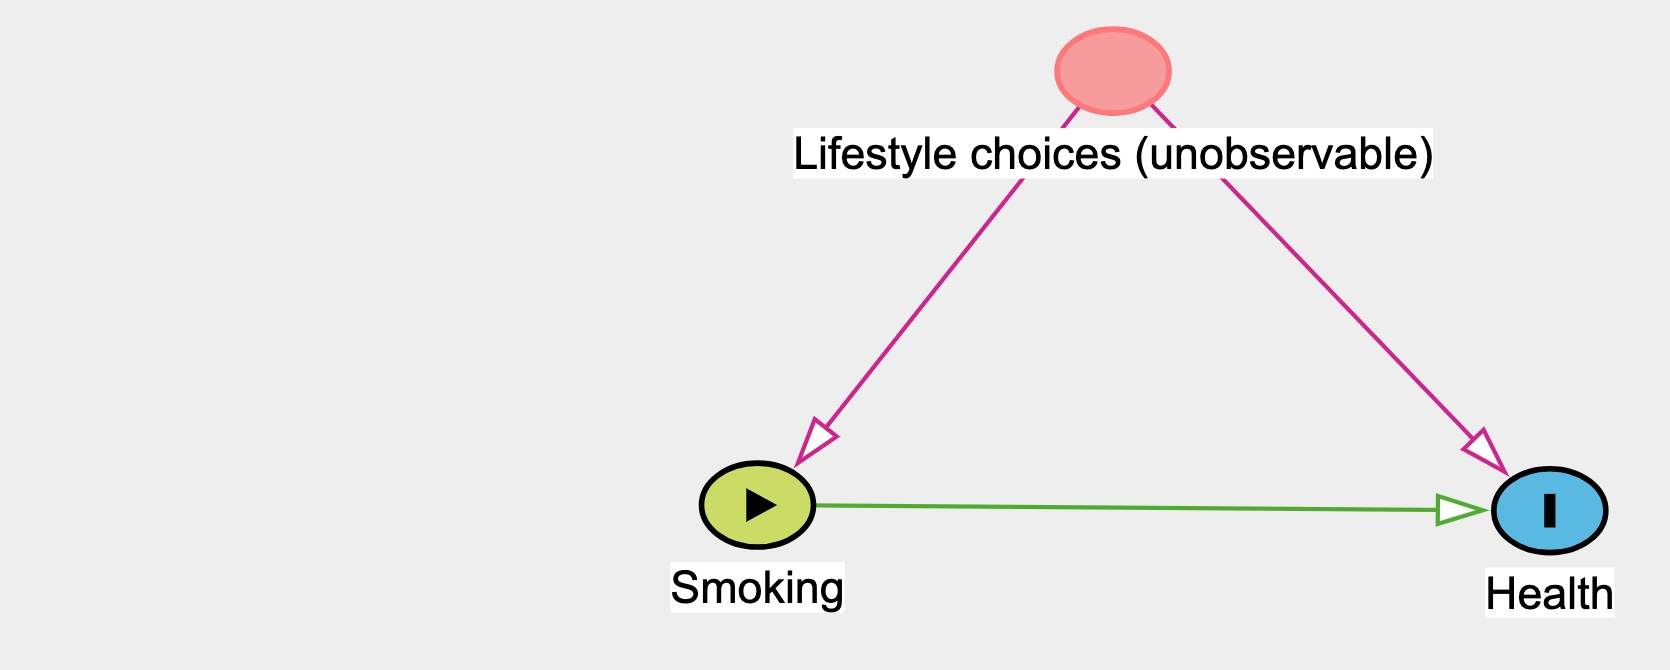
\includegraphics[width = \textwidth]{../img/smoking1}

\end{frame}
% ----------------------------------------------------

% ----------------------------------------------------
\begin{frame}
\frametitle{Methods and causal inference}
\centering

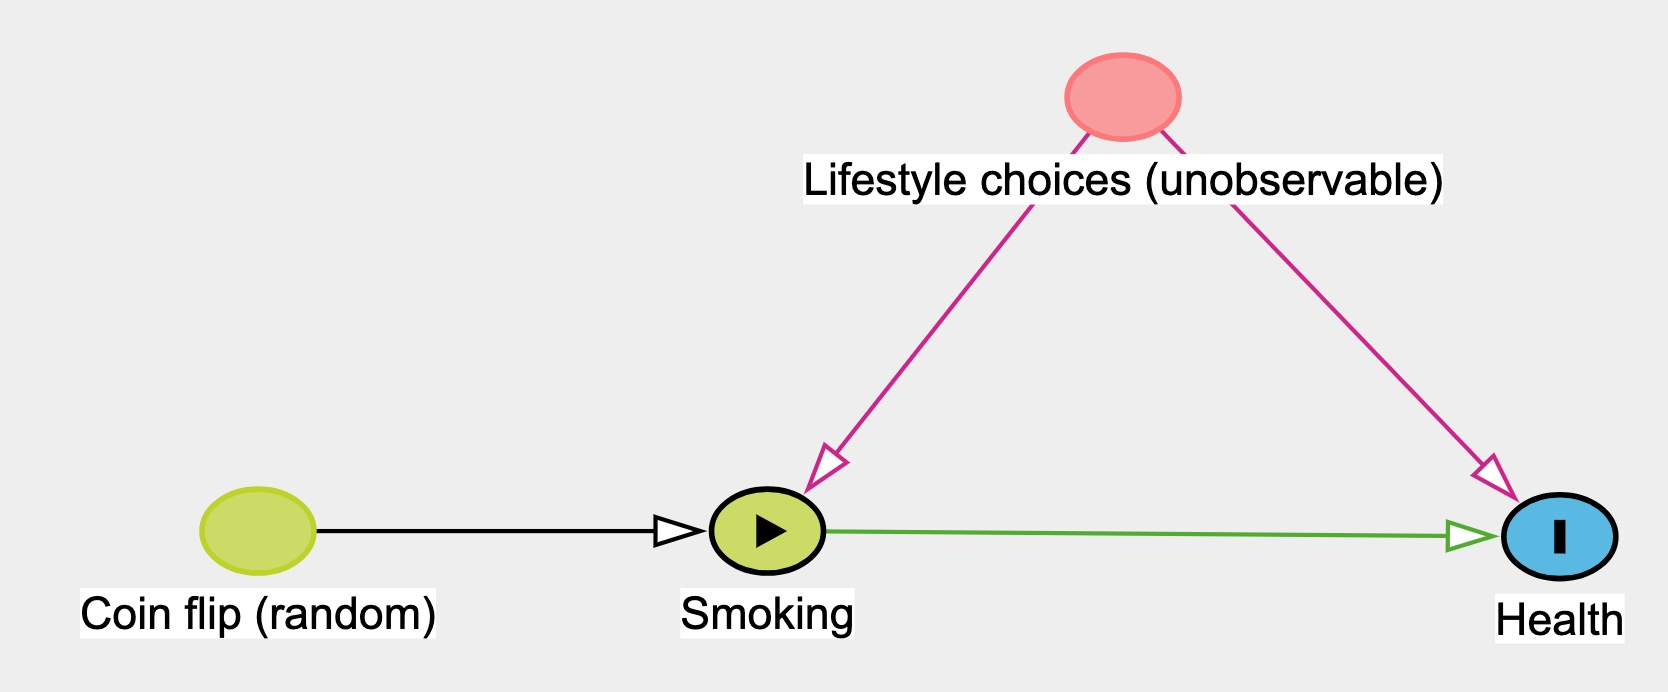
\includegraphics[width = \textwidth]{../img/smoking2}

\end{frame}
% ----------------------------------------------------

% % ----------------------------------------------------
% \begin{frame}
% \frametitle{Methods and causal inference}
% \centering
%
% \begin{itemize}
%   \item[1.] Time
%   \begin{itemize}
%     \item we can exploit changes over time in treated vs control units, e.g. imagine checking effect of good nutrition on a child who is growing anyway
%   \end{itemize}
%   \item[2.] Cut-offs
%   \begin{itemize}
%     \item sometimes something happens just when you cross a cut-off (getting into university, winning an election, a geographical border, being born Jan 1st...)
%   \end{itemize}
%   \item[3.] A third, unrelated variable
%   \begin{itemize}
%     \item you win the lottery, you get a sudden increase in disposable income
%   \end{itemize}
% \end{itemize}
%
% \end{frame}
% % ----------------------------------------------------

% ----------------------------------------------------
\begin{frame}
\frametitle{Methods and causal inference}
\centering

\begin{itemize}
  \item[-] Five techniques commonly used in causal inference
  \begin{itemize}
    \item two of them use for controlling (closing back-doors), and the other three to exploit `pre-made` causal models
    \item btw, what is controlling? when you control for Z, you remove the variation in X and Y that is \textit{explained by Z} (\href{https://www.nickchk.com/anim/Animation\%20of\%20Control.gif}{see this})
  \end{itemize}
  \item[]
  \item<2->[1.] Fixed effects
  \item<2->[2.] Difference-in-differences
  \item<2->[3.] Regression discontinuity design
  \item<2->[4.] Instrumental variables
  \item<2->[5.] Matching
\end{itemize}

\end{frame}
% ----------------------------------------------------

\section{Methods in brief}

% ----------------------------------------------------
\begin{frame}
\frametitle{Fixed effects}
\centering

\begin{itemize}
  \item The problem with covariate adjustment is that we need to \textit{observe} those variables, but we usually have unobserved confounders
  \item An strategy in that case is to try within-group comparisons, which blocks all group-wide confounding
  \item For example, imagine cases when our $U$ variable is:
  \begin{itemize}
    \item \textit{city of origin}, in an individual-level analysis; \textit{school effects} in an analyses of students grades; \textit{individual background}, in a panel survey analysis...
  \end{itemize}
  \item It corrects for \BGyellow{ecological fallacy} (esp. Simpson's paradox)
  \item Estimation: dummy variable for each group
\end{itemize}

\end{frame}
% ----------------------------------------------------

% ----------------------------------------------------
\begin{frame}
\frametitle{Fixed effects}
\centering

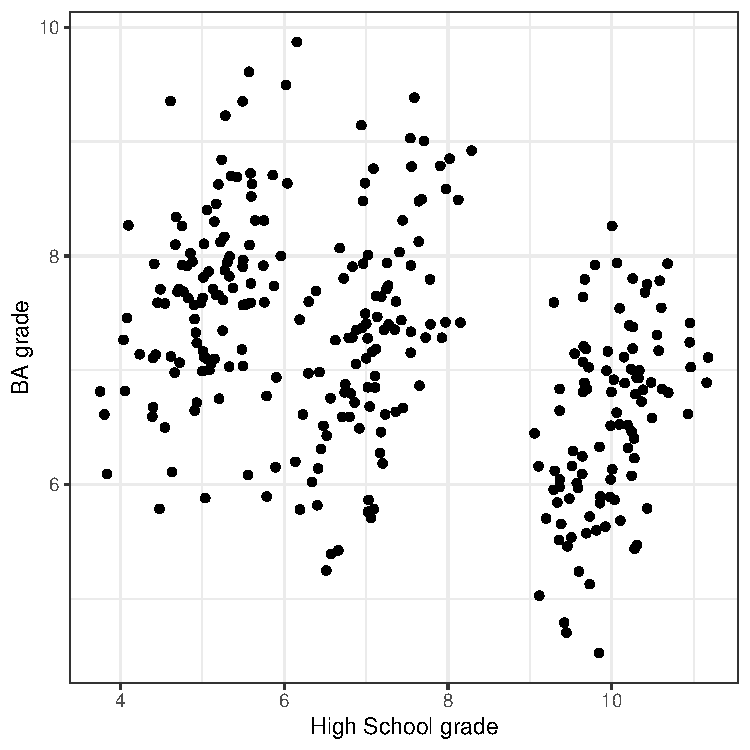
\includegraphics[width = 0.7\textwidth]{../img/fe1}

\end{frame}
% ----------------------------------------------------

% ----------------------------------------------------
\begin{frame}
\frametitle{Fixed effects}
\centering

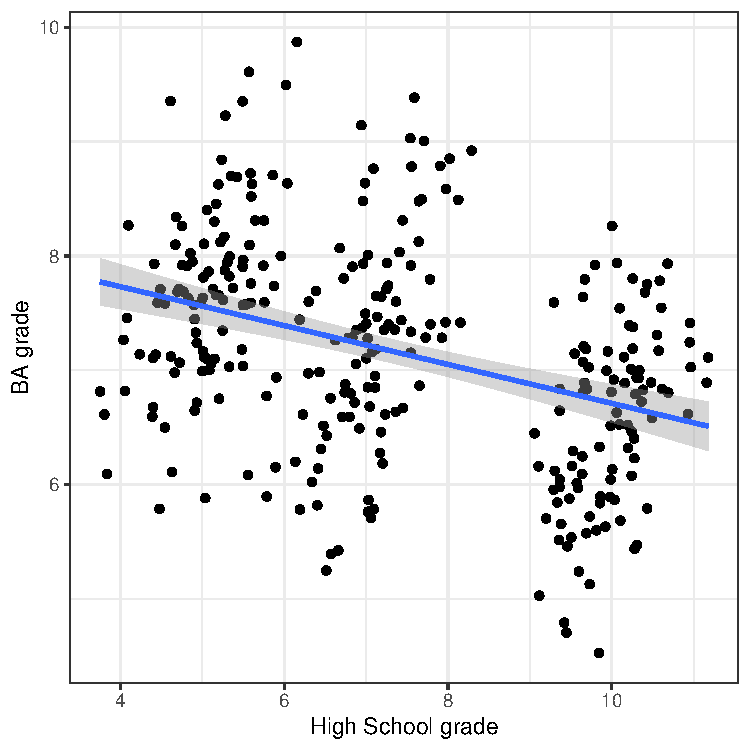
\includegraphics[width = 0.7\textwidth]{../img/fe2}

\end{frame}
% ----------------------------------------------------

% ----------------------------------------------------
\begin{frame}
\frametitle{Fixed effects}
\centering

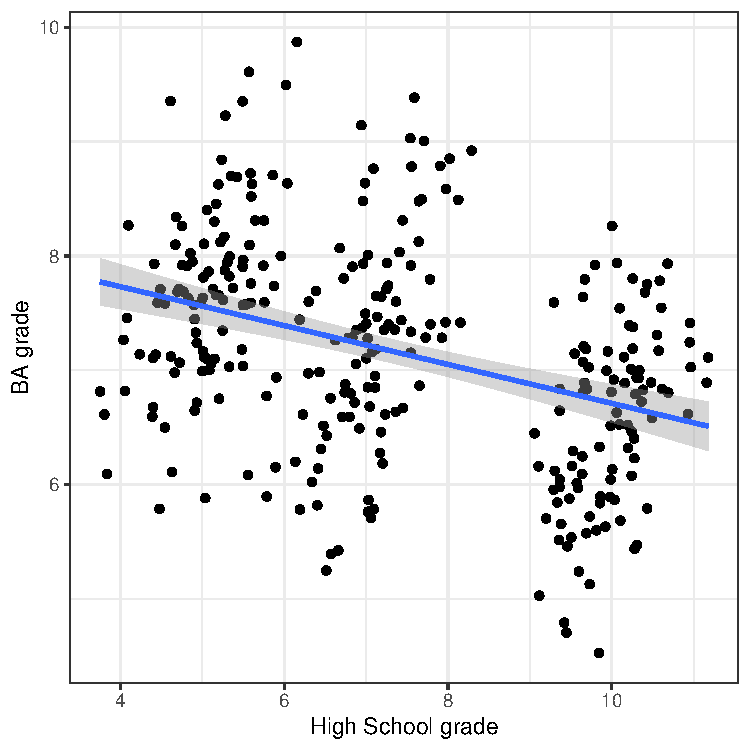
\includegraphics[width = 0.7\textwidth]{../img/fe2}

\end{frame}
% ----------------------------------------------------

% ----------------------------------------------------
\begin{frame}
\frametitle{Fixed effects}
\centering

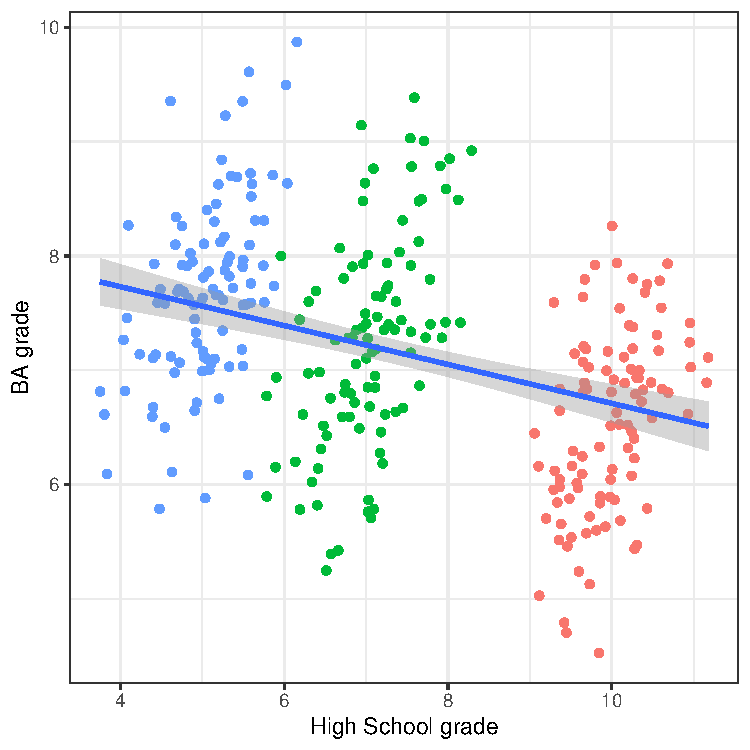
\includegraphics[width = 0.7\textwidth]{../img/fe3}

\end{frame}
% ----------------------------------------------------

% ----------------------------------------------------
\begin{frame}
\frametitle{Fixed effects}
\centering

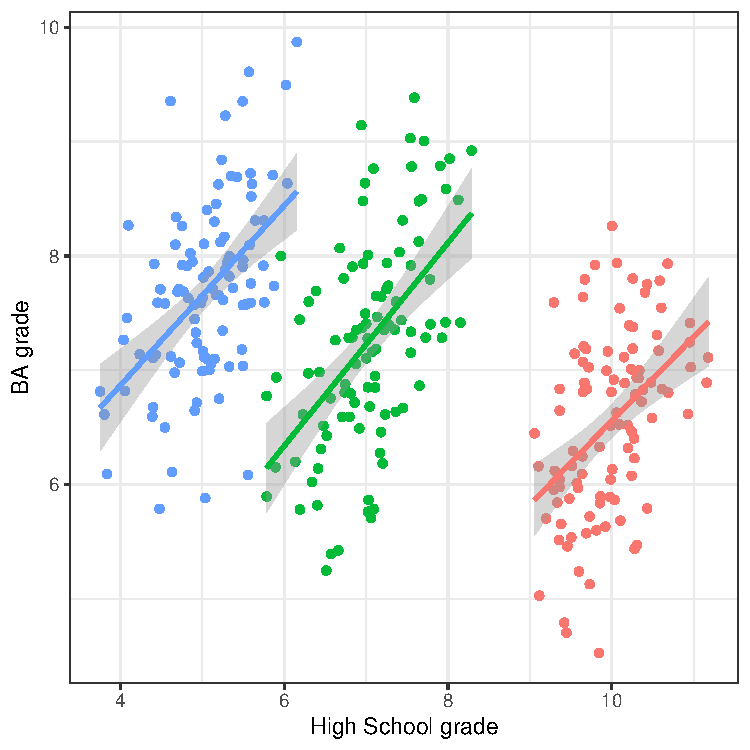
\includegraphics[width = 0.7\textwidth]{../img/fe4}

\end{frame}
% ----------------------------------------------------

% ----------------------------------------------------
\begin{frame}
\frametitle{Fixed effects}
\centering

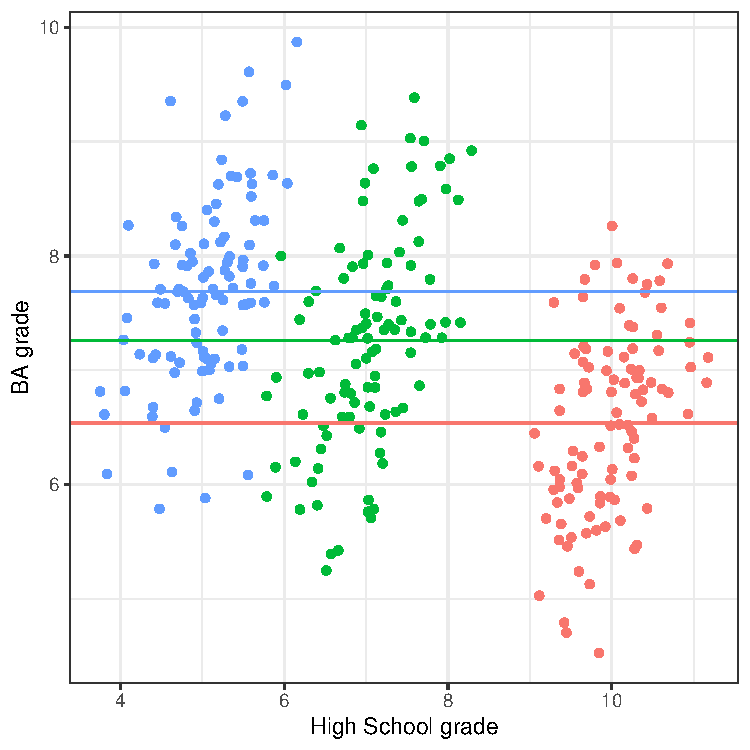
\includegraphics[width = 0.7\textwidth]{../img/fe5}

\end{frame}
% ----------------------------------------------------

% ----------------------------------------------------
\begin{frame}
\frametitle{Fixed effects}
\centering

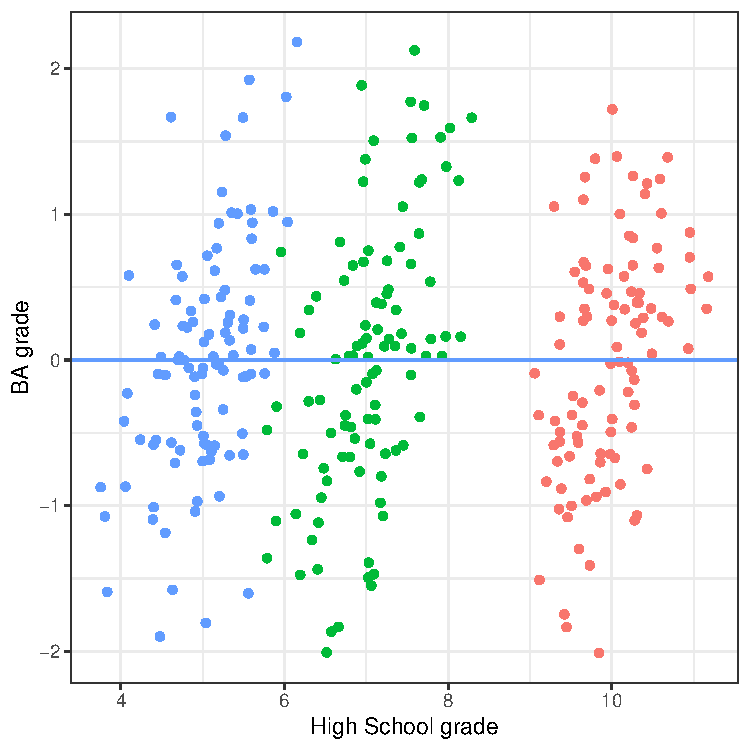
\includegraphics[width = 0.7\textwidth]{../img/fe6}

\end{frame}
% ----------------------------------------------------

% ----------------------------------------------------
\begin{frame}
\frametitle{Fixed effects}
\centering

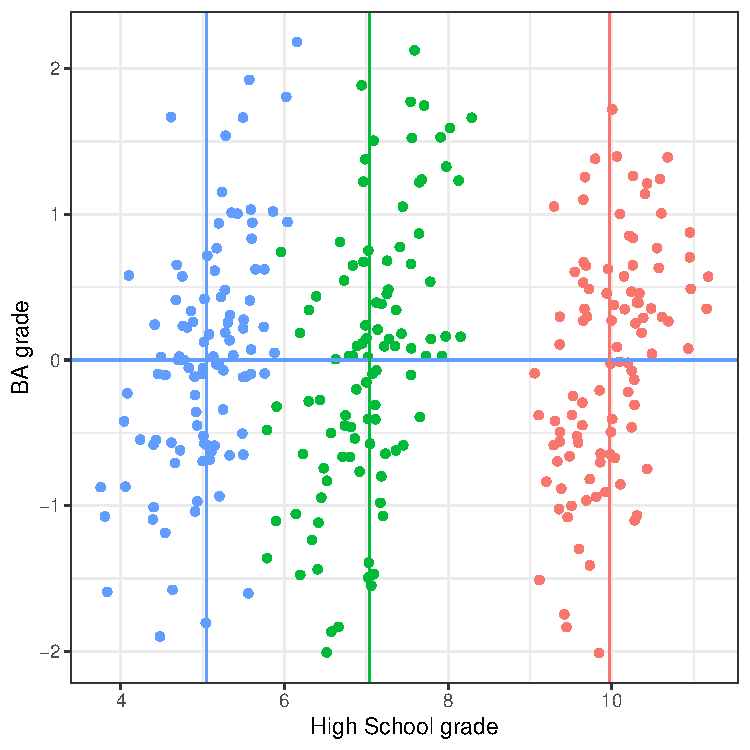
\includegraphics[width = 0.7\textwidth]{../img/fe7}

\end{frame}
% ----------------------------------------------------

% ----------------------------------------------------
\begin{frame}
\frametitle{Fixed effects}
\centering

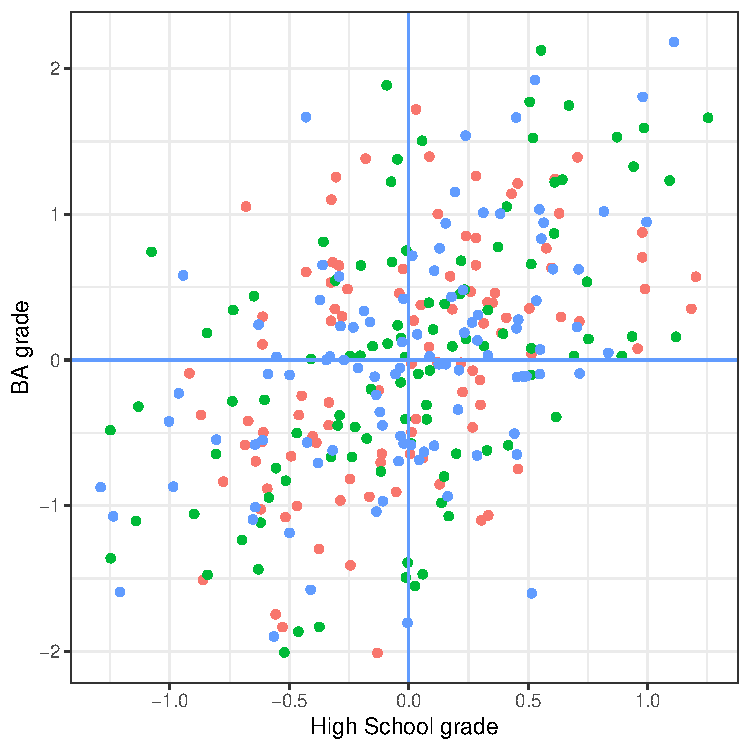
\includegraphics[width = 0.7\textwidth]{../img/fe8}

\end{frame}
% ----------------------------------------------------

% ----------------------------------------------------
\begin{frame}
\frametitle{Fixed effects}
\centering

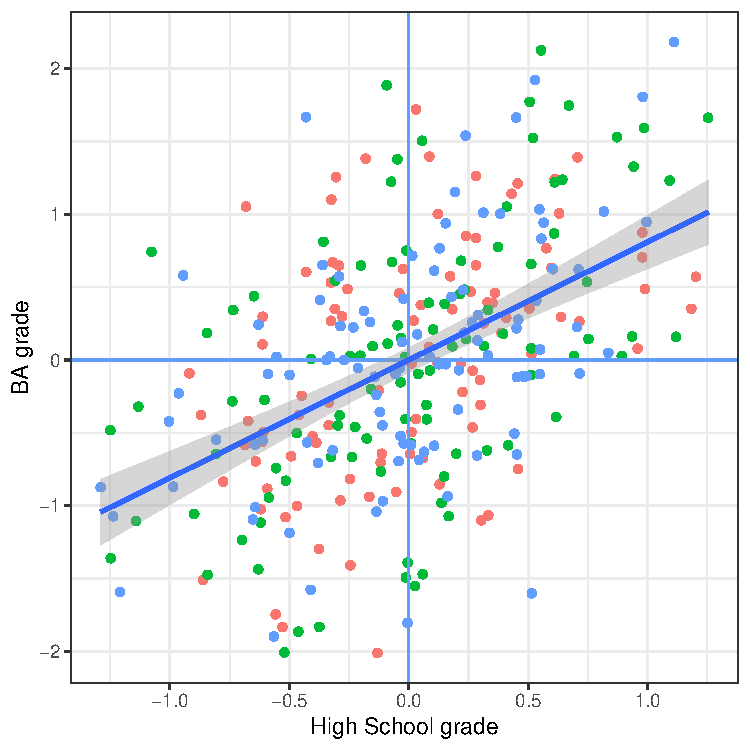
\includegraphics[width = 0.7\textwidth]{../img/fe9}

\end{frame}
% ----------------------------------------------------

% ----------------------------------------------------
\begin{frame}
\frametitle{Difference-in-differences}
\centering

\begin{itemize}
  \item Treatments usually occur at a particular moment in time, e.g.:
    \begin{itemize}
      \item Minimum wage increase, terrorist attacks, influx of refugees, ...
    \end{itemize}
  \item A naive idea would be to compare how it was \textit{before} the treatment with how it is \textit{after} the treatment, right?
    \begin{itemize}
      \item e.g. in municipalities that removed Francoist streets, how much did Vox grow between 2016 and 2019?
    \end{itemize}
  \item or we could just compare treated vs control \textit{after} treatment
    \begin{itemize}
      \item e.g. did Vox get more votes in 2019 in municipalities that removed F streets?
    \end{itemize}
  \item DiD idea: use a control group that works as a \BGyellow{counterfactual} for how much would $Y$ have changed without treatment
  \end{itemize}

\end{frame}
% ----------------------------------------------------

% ----------------------------------------------------
\begin{frame}
\frametitle{Difference-in-differences}
\centering

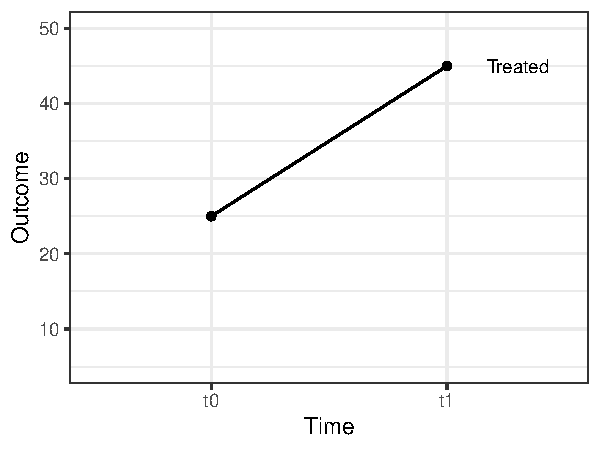
\includegraphics[width = 0.8\textwidth]{../img/did1}

\end{frame}
% ----------------------------------------------------

% ----------------------------------------------------
\begin{frame}
\frametitle{Difference-in-differences}
\centering

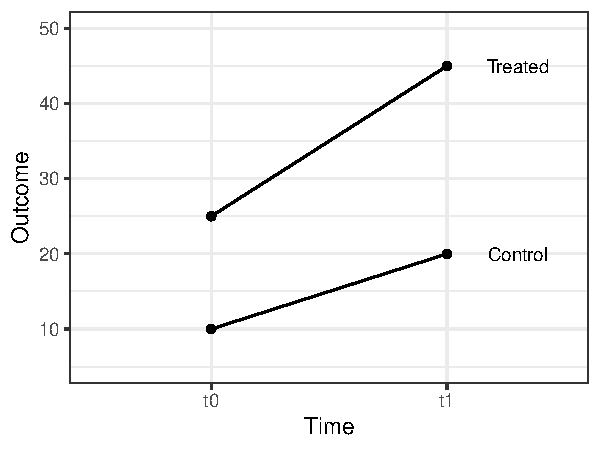
\includegraphics[width = 0.8\textwidth]{../img/did2}

\end{frame}
% ----------------------------------------------------

% ----------------------------------------------------
\begin{frame}
\frametitle{Difference-in-differences}
\centering

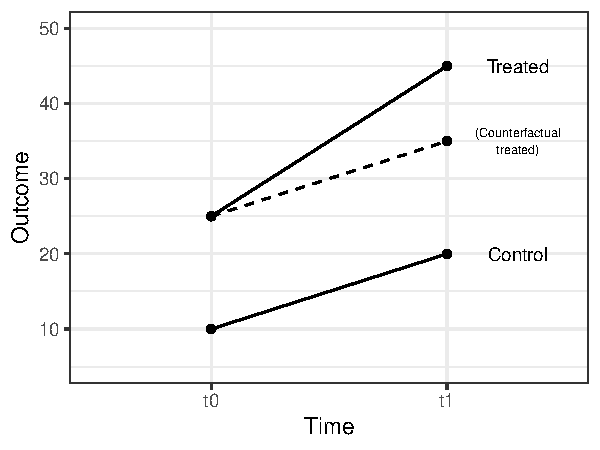
\includegraphics[width = 0.8\textwidth]{../img/did3}

\end{frame}
% ----------------------------------------------------

% ----------------------------------------------------
\begin{frame}
\frametitle{Difference-in-differences}
\centering

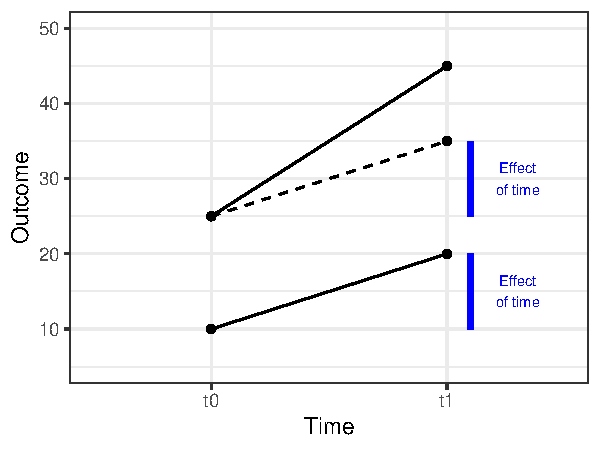
\includegraphics[width = 0.8\textwidth]{../img/did4}

\end{frame}
% ----------------------------------------------------

% ----------------------------------------------------
\begin{frame}
\frametitle{Difference-in-differences}
\centering

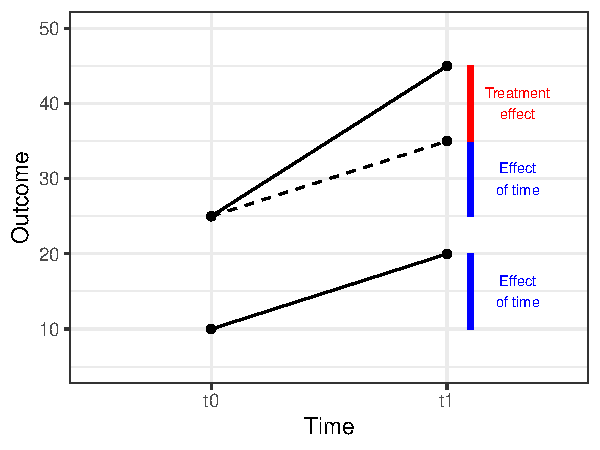
\includegraphics[width = 0.8\textwidth]{../img/did5}

\end{frame}
% ----------------------------------------------------

% ----------------------------------------------------
\begin{frame}
\frametitle{Difference-in-differences estimation}
\centering

\begin{itemize}
  \item You normally estimate it using a regression model (OLS or logit, depending on the outcome) on panel data
  \begin{itemize}
    \item each unit has one observation per period (at least, before/after treatment)
  \end{itemize}
  \item Variables: time, group (treated or not), and their interaction
\end{itemize}

\begin{equation}
\begin{split}
    Y_{it} =&  \beta_0 + \beta_1 Treated_{i} + \beta_2 After_{t} +\\
    &\beta_3 (Treated_{i} \times After_{t}) + \beta^\top \mathbf{x}_{i} + \epsilon_{it}
\end{split}
\end{equation}

\begin{itemize}
  \item \BGyellow{Key assumption}: control group is a good counterfactual
  \begin{itemize}
    \item checking parallel trends assumption
  \end{itemize}
\end{itemize}

\end{frame}
% ----------------------------------------------------

% ----------------------------------------------------
\begin{frame}
\frametitle{Regression discontinuity design}
\centering

\begin{itemize}
  \item RDD works well when assignment into treatment depends on a cutoff along a \BGyellow{running variable}
  \begin{itemize}
    \item Do incumbent politicians have an electoral advantage? (vote share)
    \item What is the effect of being drafted into the military? (birth year)
    \item Effect of national policies in ethnic identification in Africa? (distance to colonial borders)
  \end{itemize}
  \item The source of the exogenous variation:
  \begin{itemize}
    \item Although many variables confound the relationships between $X$ and $Y$, nothing should be too different \textit{around the cutoff} between treatment and control groups (local randomization assumption)
  \end{itemize}
\end{itemize}

\end{frame}
% ----------------------------------------------------

% ----------------------------------------------------
\begin{frame}
\frametitle{Regression discontinuity design}
\centering

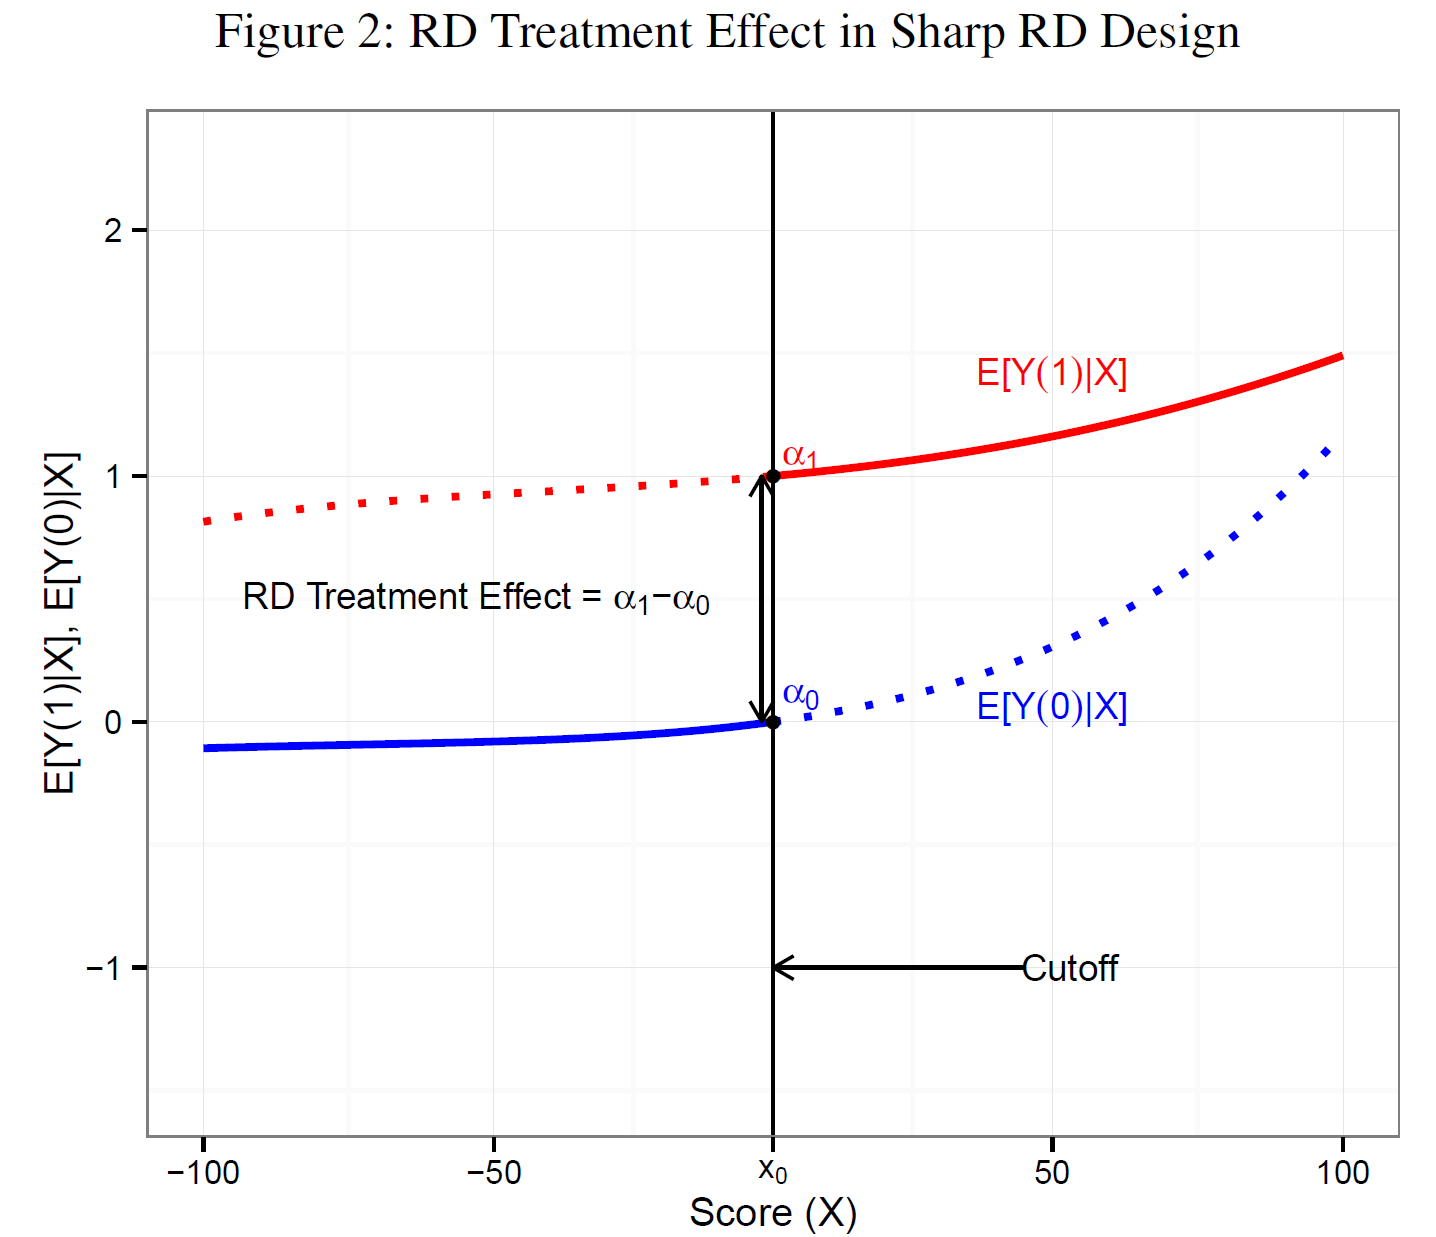
\includegraphics[width = 0.8\textwidth]{../img/rdd_teffect}

\end{frame}
% ----------------------------------------------------

% ----------------------------------------------------
\begin{frame}
\frametitle{Regression discontinuity design}
\centering

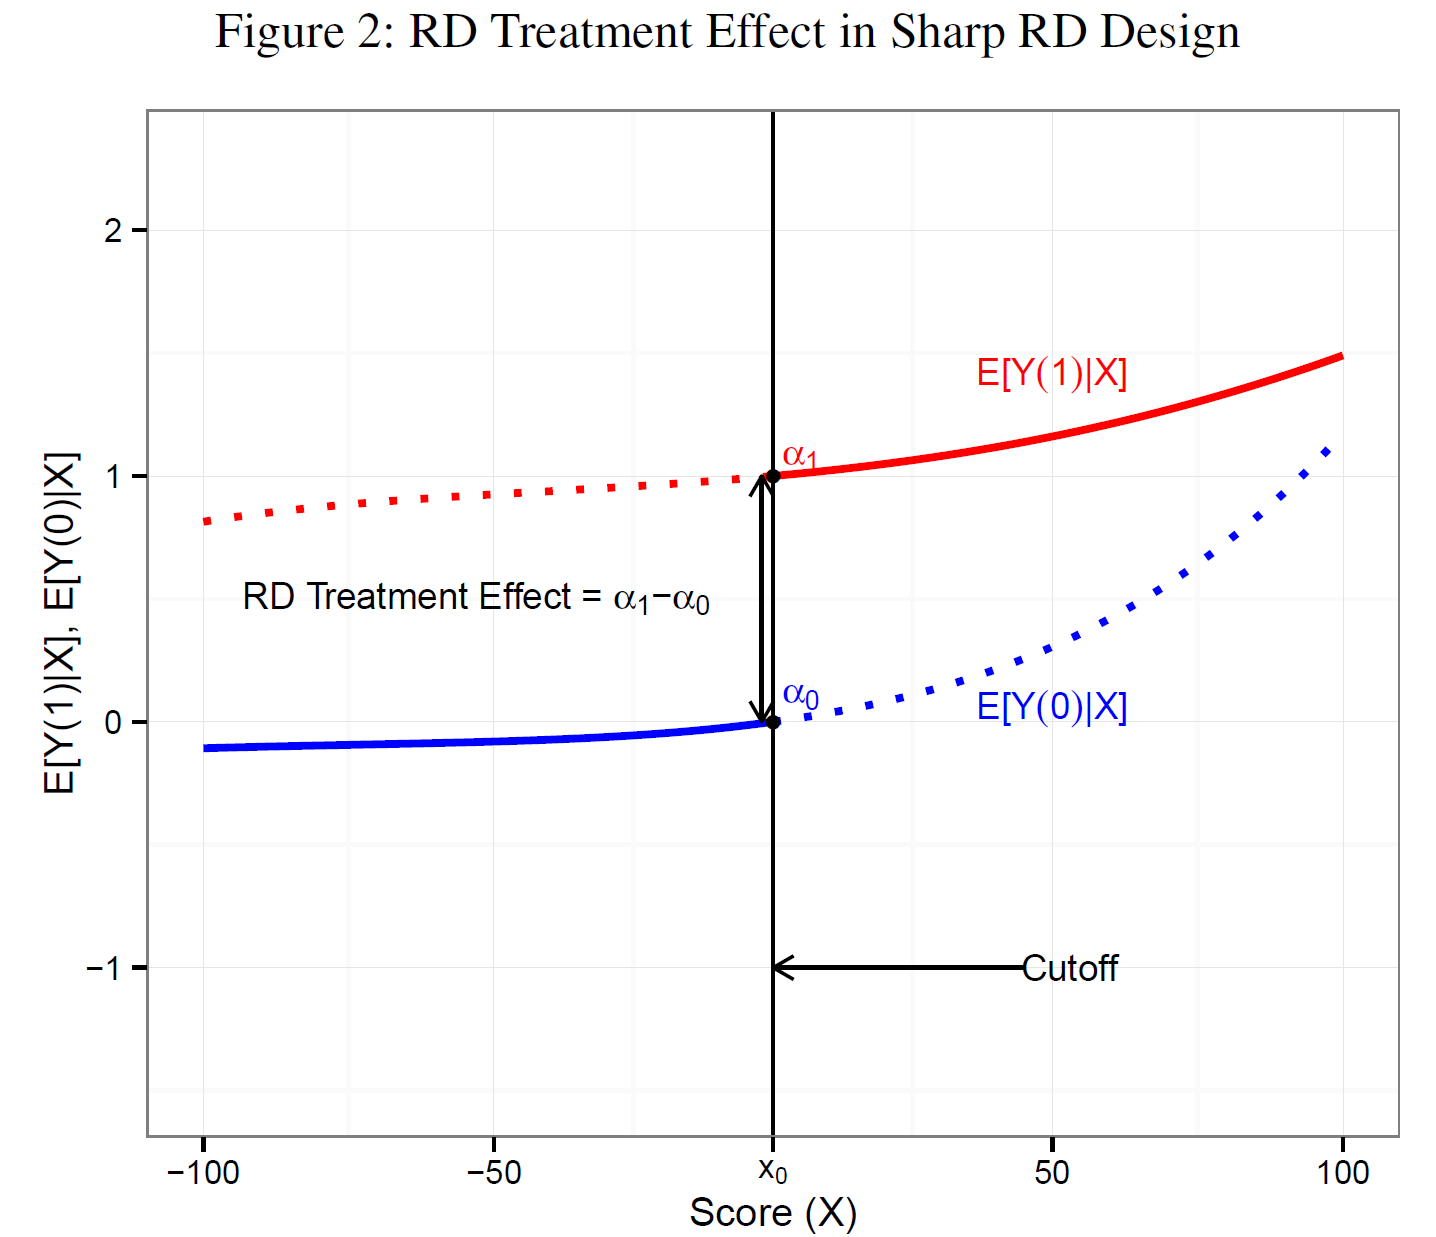
\includegraphics[width = 0.8\textwidth]{../img/rdd_teffect}

\end{frame}
% ----------------------------------------------------

% ----------------------------------------------------
\begin{frame}
\frametitle{Regression discontinuity design}
\centering

\begin{itemize}
  \item \BGyellow{Key assumption}: other confounders also vary along the running variable, but are independent to the \textit{jump over cutoff}
\end{itemize}

\vspace{50pt}

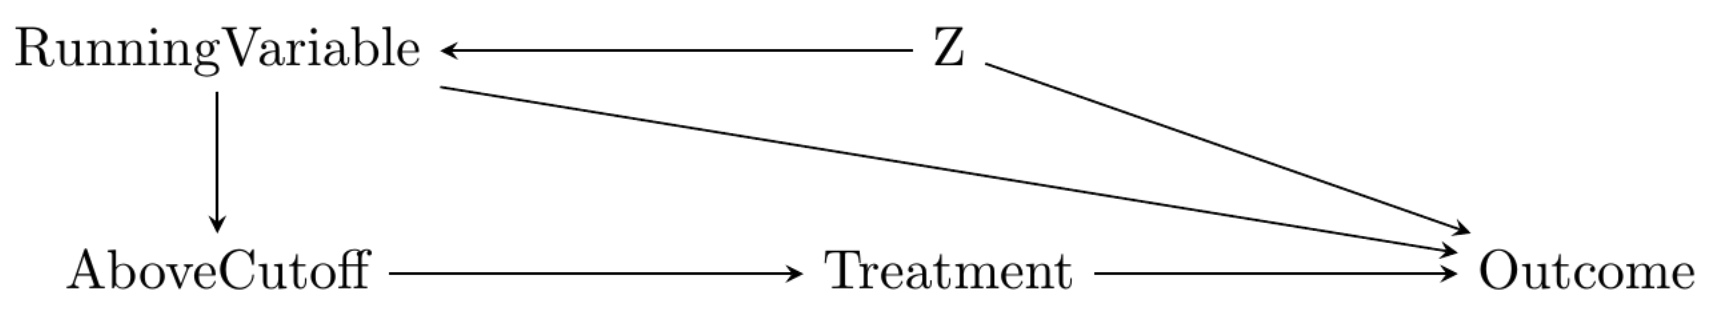
\includegraphics[width = \textwidth]{../img/rdd_dag}

\vspace{15pt}

{\scriptsize Huntington-Klein, \textit{The Effect}, p.508}

\end{frame}
% ----------------------------------------------------

% ----------------------------------------------------
\begin{frame}
\frametitle{RDD estimates the \BGyellow{LATE}}
\centering

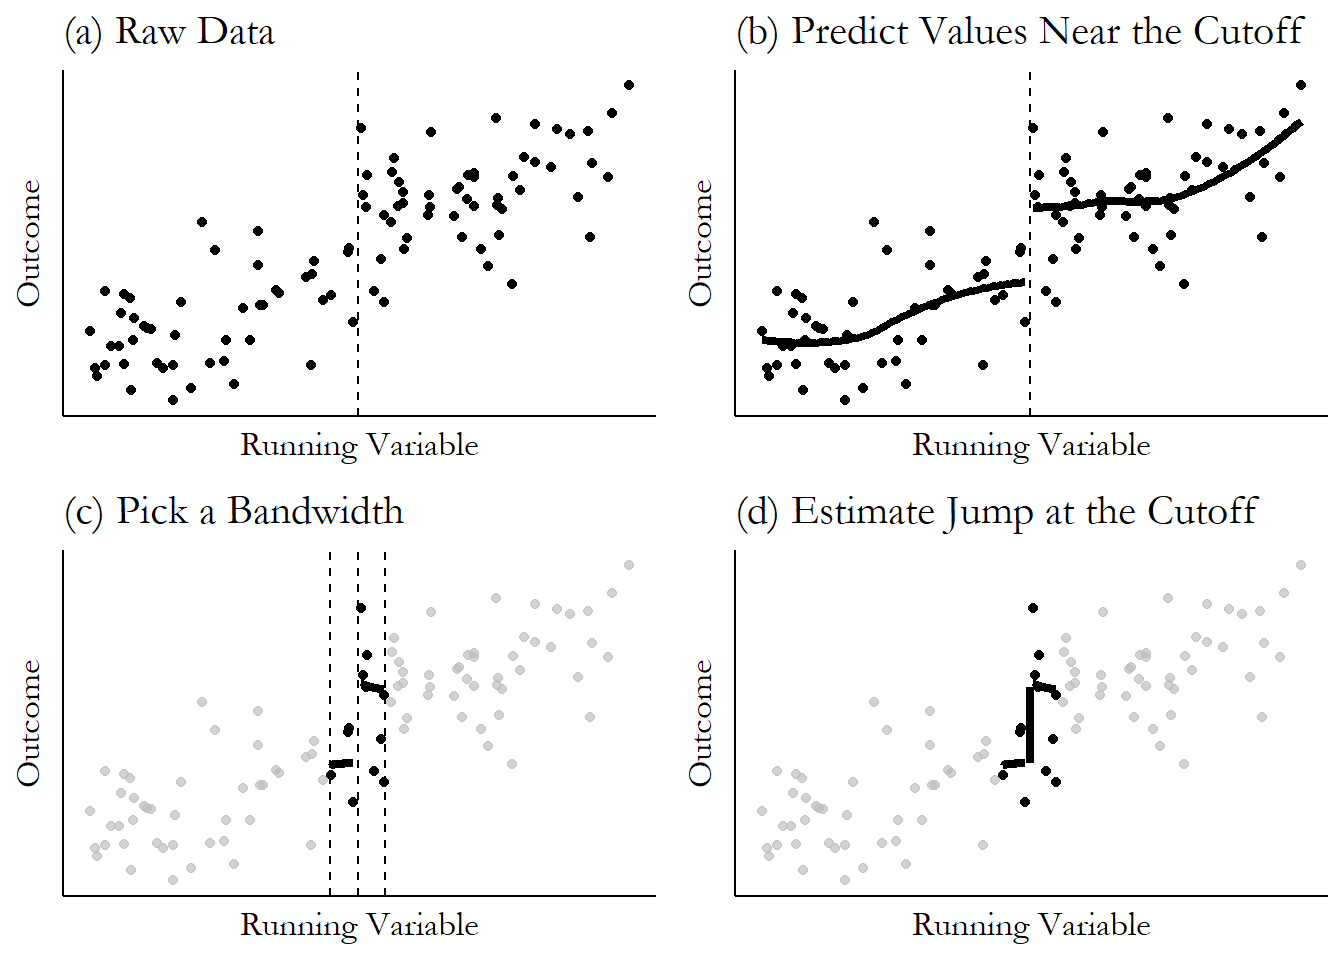
\includegraphics[width = \textwidth]{../img/rdd_procedure}

\end{frame}
% ----------------------------------------------------

% ----------------------------------------------------
\begin{frame}
\frametitle{Threats in RDD}
\centering

\begin{itemize}
  \item \BGyellow{Outcome $\rightarrow$ cutoff}: what we study might actually affect cutoff (e.g. colonial borders and ethnic ID)
  \begin{itemize}
    \item could also be a case of confounding, cutoff $\leftarrow Z \rightarrow$ outcome
  \end{itemize}
  \item \BGyellow{Precise sorting}: maybe something is \textit{actually} affecting sorting around the cutoff (next example)
  \item Causal effect \BGyellow{independent of treatment}: being above/below cutoff affects $Y$ independent of the treatment we're interesting in
\end{itemize}

\end{frame}
% ----------------------------------------------------

% ----------------------------------------------------
\begin{frame}
\frametitle{Threats in RDD: precise sorting}
\centering

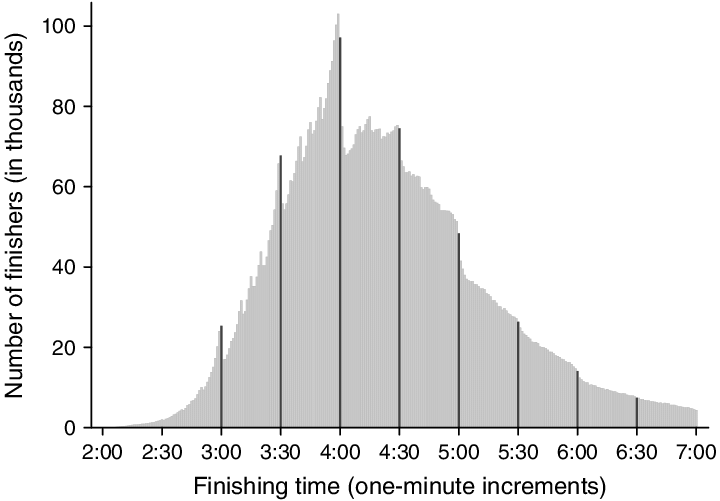
\includegraphics[width = \textwidth]{../img/marathon_finishing_times}

\end{frame}
% ----------------------------------------------------

% ----------------------------------------------------
\begin{frame}
\frametitle{Instrumental variables}
\centering

\begin{tikzpicture}[every text node part/.style={align=center}, scale = 0.75]
\node (r) at (0,0){\texttt{random}};
\node (y) at (7,0){Y};
\node (x) at (3.5,0){X};
\node (u) at (5,1.5){U};
\draw[->] (r) -- (x);
\draw[->] (x) -- (y);
\draw[->, dashed] (u) -- (y);
\draw[->, dashed] (u) -- (x);
\end{tikzpicture}

\begin{itemize}
  \item Probably closest idea to a `natural experiment'
\end{itemize}

\end{frame}
% ----------------------------------------------------

% ----------------------------------------------------
\begin{frame}
\frametitle{Instrumental variables}
\centering

\begin{itemize}
  \item Find an exogenous source of variation in the treatment variable
  \begin{itemize}
    \item e.g., we want to know the effect of protests on government action, and we use \textit{rainfall} as an instrument
  \end{itemize}
  \item Isolate that variation and use it to identify the causal effect
  \begin{itemize}
    \item two-stage least squares, or 2SLS
  \end{itemize}
  \item[]
  \item<2->[] \textbf{Assumptions:}
  \item<2-> \BGyellow{Relevance}: the instrument explains at least some part of the treatment variable
  \item<2-> Validity or \BGyellow{exclusion restriction}: no back door paths between the instrument and the outcome
\end{itemize}

\end{frame}
% ----------------------------------------------------

% ----------------------------------------------------
\begin{frame}
\frametitle{Matching}
\centering

\begin{itemize}
  \item Main idea behind matching: adding control variables is \textit{not the only way} to control / close back doors
  \item When you use a subset selecting on a variable, you are controlling for that variable
  \begin{itemize}
    \item e.g. if you analyze $income \leftarrow education$ and only use data from individuals who grew up in big cities, you are already controlling for urban/rural
  \end{itemize}
  \item Matching builds on this, and it is essentially about keeping in the same only comparable observations, or \textit{matched pairs}
  \item \href{https://www.nickchk.com/anim/Animation\%20of\%20Matching.gif}{Example of $Y \leftarrow Treatment$ matching on $X$}
\end{itemize}

\end{frame}
% ----------------------------------------------------

% ----------------------------------------------------
\begin{frame}
\frametitle{Matching}
\centering

\begin{itemize}
  \item Normally you match treated units on a few control units (so you would get the \textbf{ATT})
  \item But in some cases you do the opposite, because you have more treated units that control (and you get the \textbf{ATC})
  \begin{itemize}
    \item Example from Ukraine survey paper
  \end{itemize}
  \item Two basic approaches:
  \begin{itemize}
    \item \BGyellow{Distance matching:} you select observations that have similar values on the matching variables
    \item \BGyellow{Propensity score matching:} we estimate the probability of being treated based on a set of variables, and then control/subset for that propensity score
  \end{itemize}
\end{itemize}

\end{frame}
% ----------------------------------------------------



% ----------------------------------------------------
\begin{frame}
\frametitle{Overall inference strategy}
\centering

\begin{itemize}
  \item In ideal experimental setting, we actually don't need any sophisticated statistics
  \begin{itemize}
    \item We can just compare the \textit{mean} of the treatment group and the \textit{mean} of the control group, that's it
  \end{itemize}
  \item<2-> In observational data, these two types of tools (controlling + exploiting exogenous variation) are often used in combination
  \item<2-> But \textbf{always remember} these methods \textbf{depend} on a \textbf{causal model}
  \item<2-> Let's look at an example {\footnotesize (from Huntington-Klein \textit{The Effect}, kind of)}
\end{itemize}

\end{frame}
% ----------------------------------------------------

% ----------------------------------------------------
\begin{frame}
\frametitle{Controlling \textbf{and} exploting exogeneity}
\centering

\begin{itemize}
  \item Q: \textbf{Does pollution determine transport choice?}
  \item And say we are going to observe variation across \textit{days}
  \begin{itemize}
    \item Outcome: car driving
    \item Treatment: pollution levels
  \end{itemize}
  \item Clear problem of endogeneity, no? {\footnotesize (driving in $t_{-1}$, economic activity, etc)}
  % \item \BGyellow{Z} $\rightarrow$ Pollution {\color{red}{$\rightarrow$}} Driving $\leftarrow$ Z
\end{itemize}

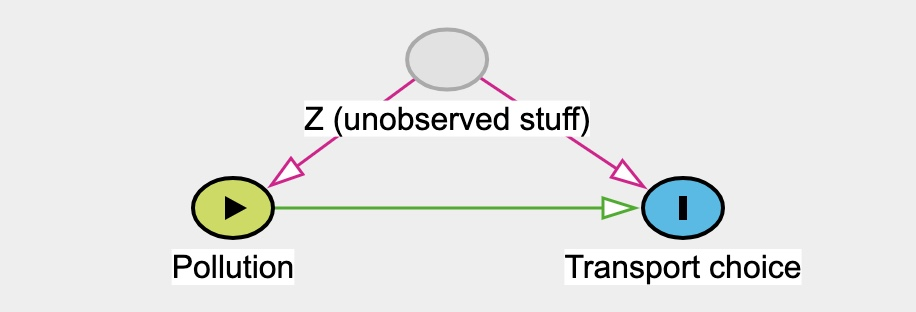
\includegraphics[width = 0.75\textwidth]{../img/pollution_dag}

\end{frame}
% ----------------------------------------------------

% ----------------------------------------------------
\begin{frame}
\frametitle{Controlling \textbf{and} exploting exogeneity}
\centering

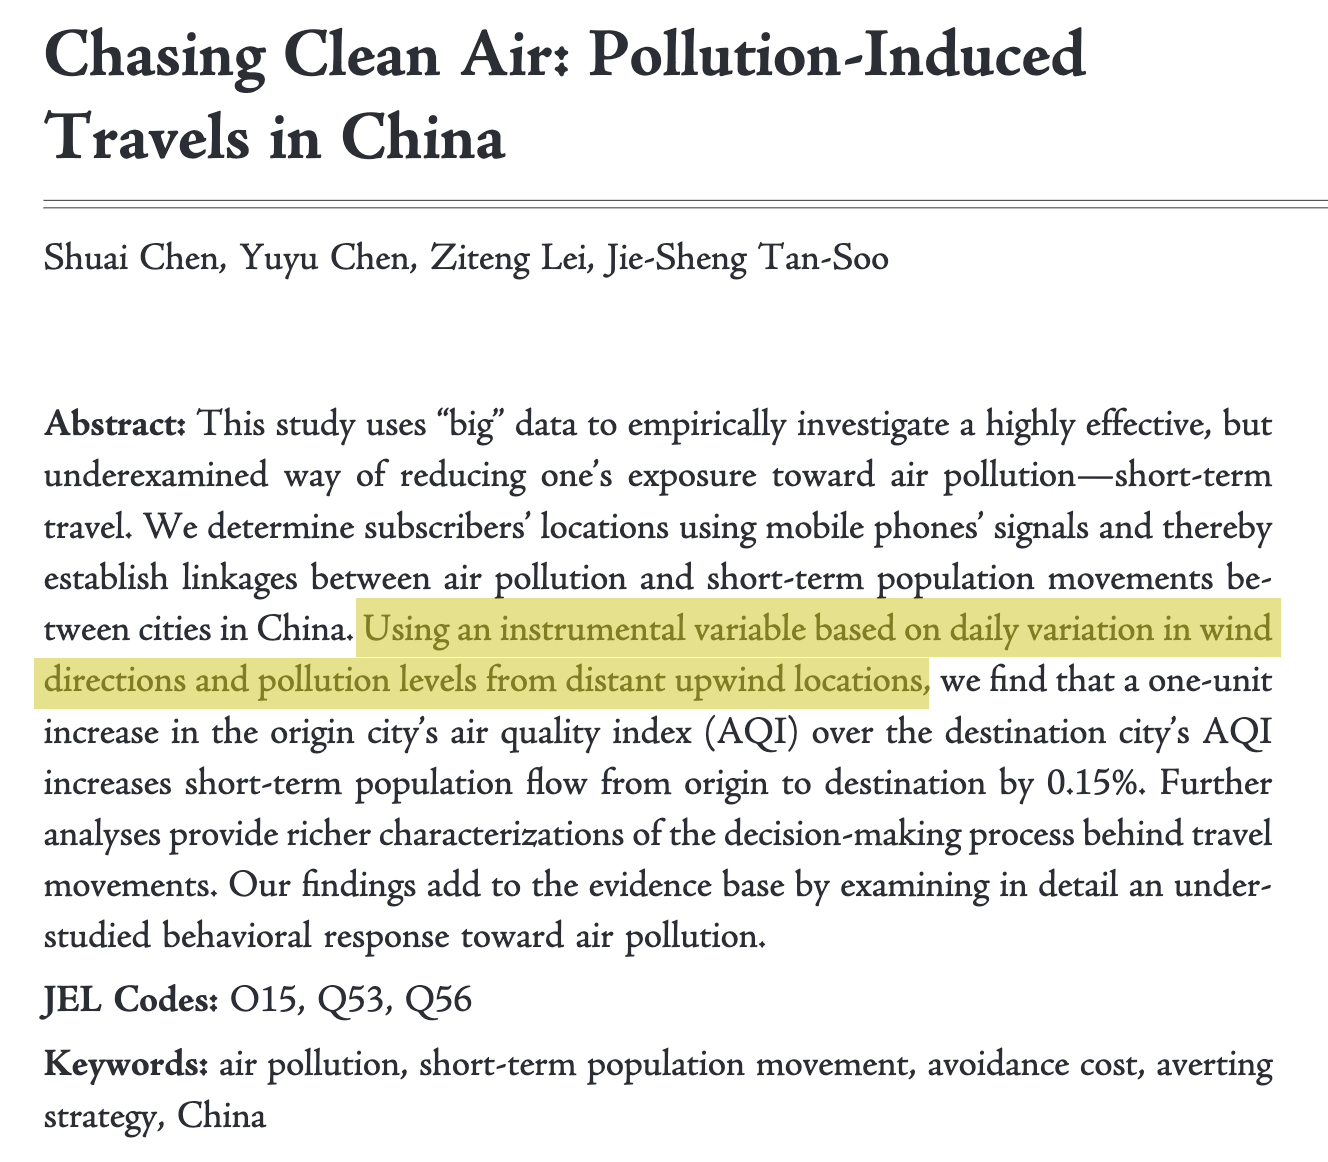
\includegraphics[width = 0.9\textwidth]{../img/china_pollution}

\end{frame}
% ----------------------------------------------------

% ----------------------------------------------------
\begin{frame}
\frametitle{Controlling \textbf{and} exploting exogeneity}
\centering

\begin{itemize}
  \item But it's not enough with wind direction, no?
\end{itemize}

\vspace{30pt}

\uncover<2->{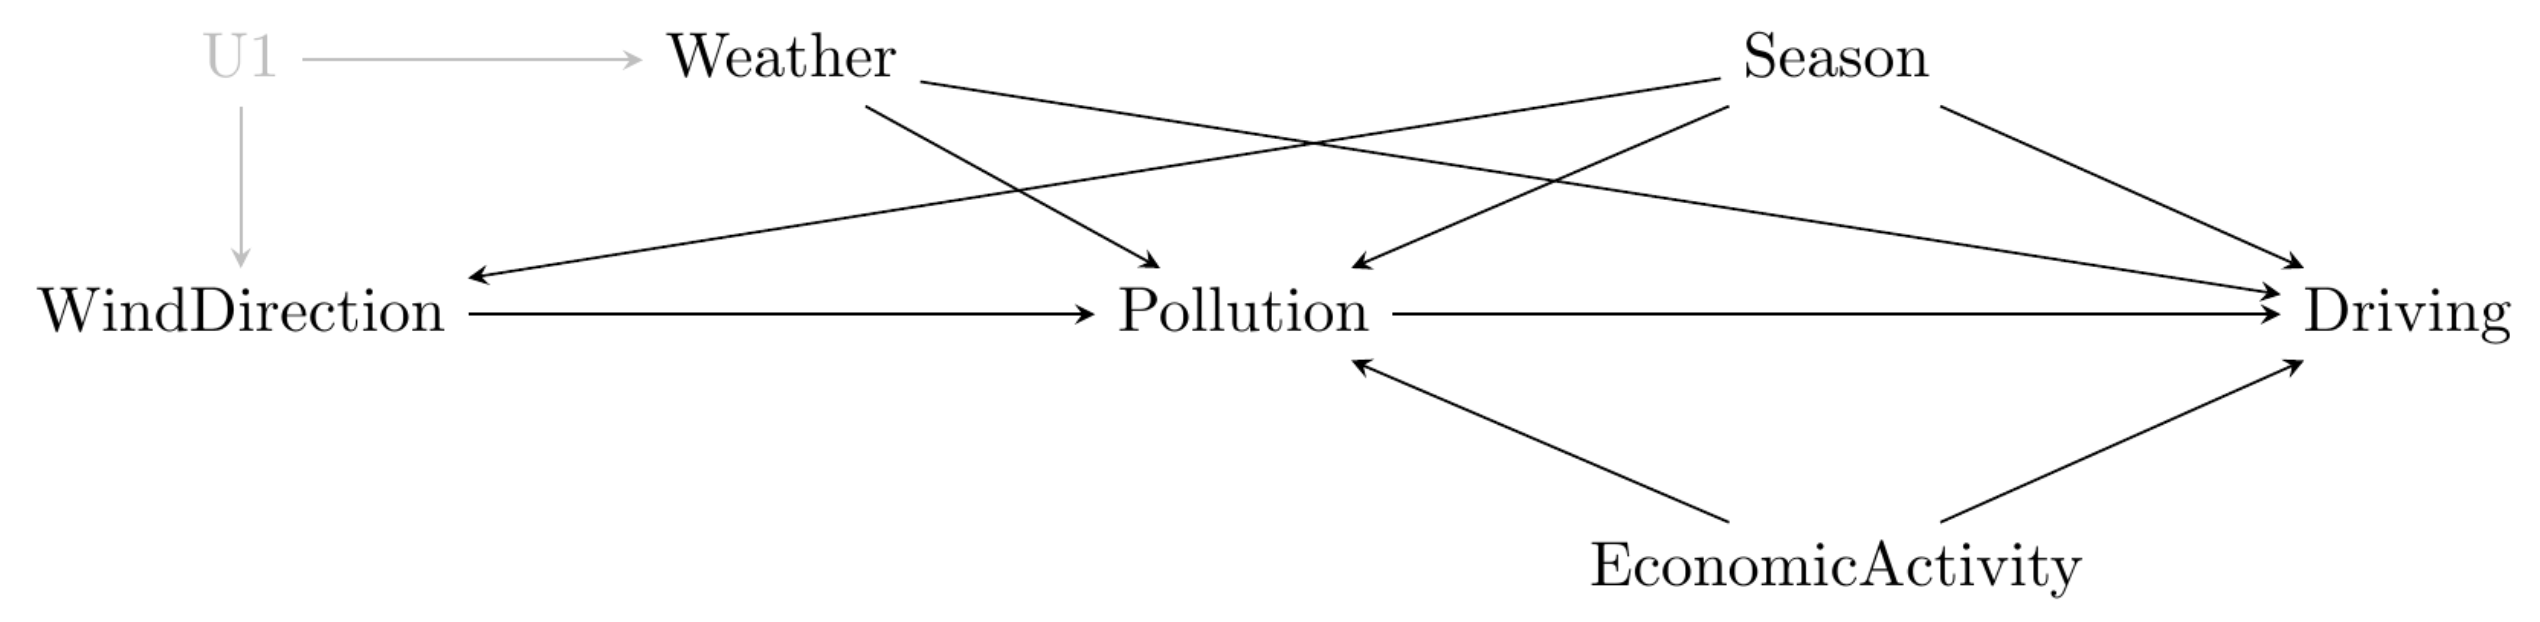
\includegraphics[width = \textwidth]{../img/china_pollution_dag}}

\begin{itemize}
  \item<2->[] (And city, in this case)
\end{itemize}

\end{frame}
% ----------------------------------------------------

% ----------------------------------------------------
\begin{frame}
\frametitle{Controlling \textbf{and} exploting exogeneity}
\centering

\begin{itemize}
  \item So in this case, we need to do two things:
  \item[1.] Exploit exogenous variation
  \begin{itemize}
    \item In this case, using an instrumental variables approach, which isolates the variation in pollution which is explained by variation in wind direction
  \end{itemize}
  \item<2->[2.] \textit{And} control for weather, season, and city
  \begin{itemize}
    \item Using a regression with control variables, or matching, or fixed effects
  \end{itemize}
\end{itemize}

\end{frame}
% ----------------------------------------------------

\section{Paper discussion}

% ----------------------------------------------------
\begin{frame}
\frametitle{Paper discussion}
\centering

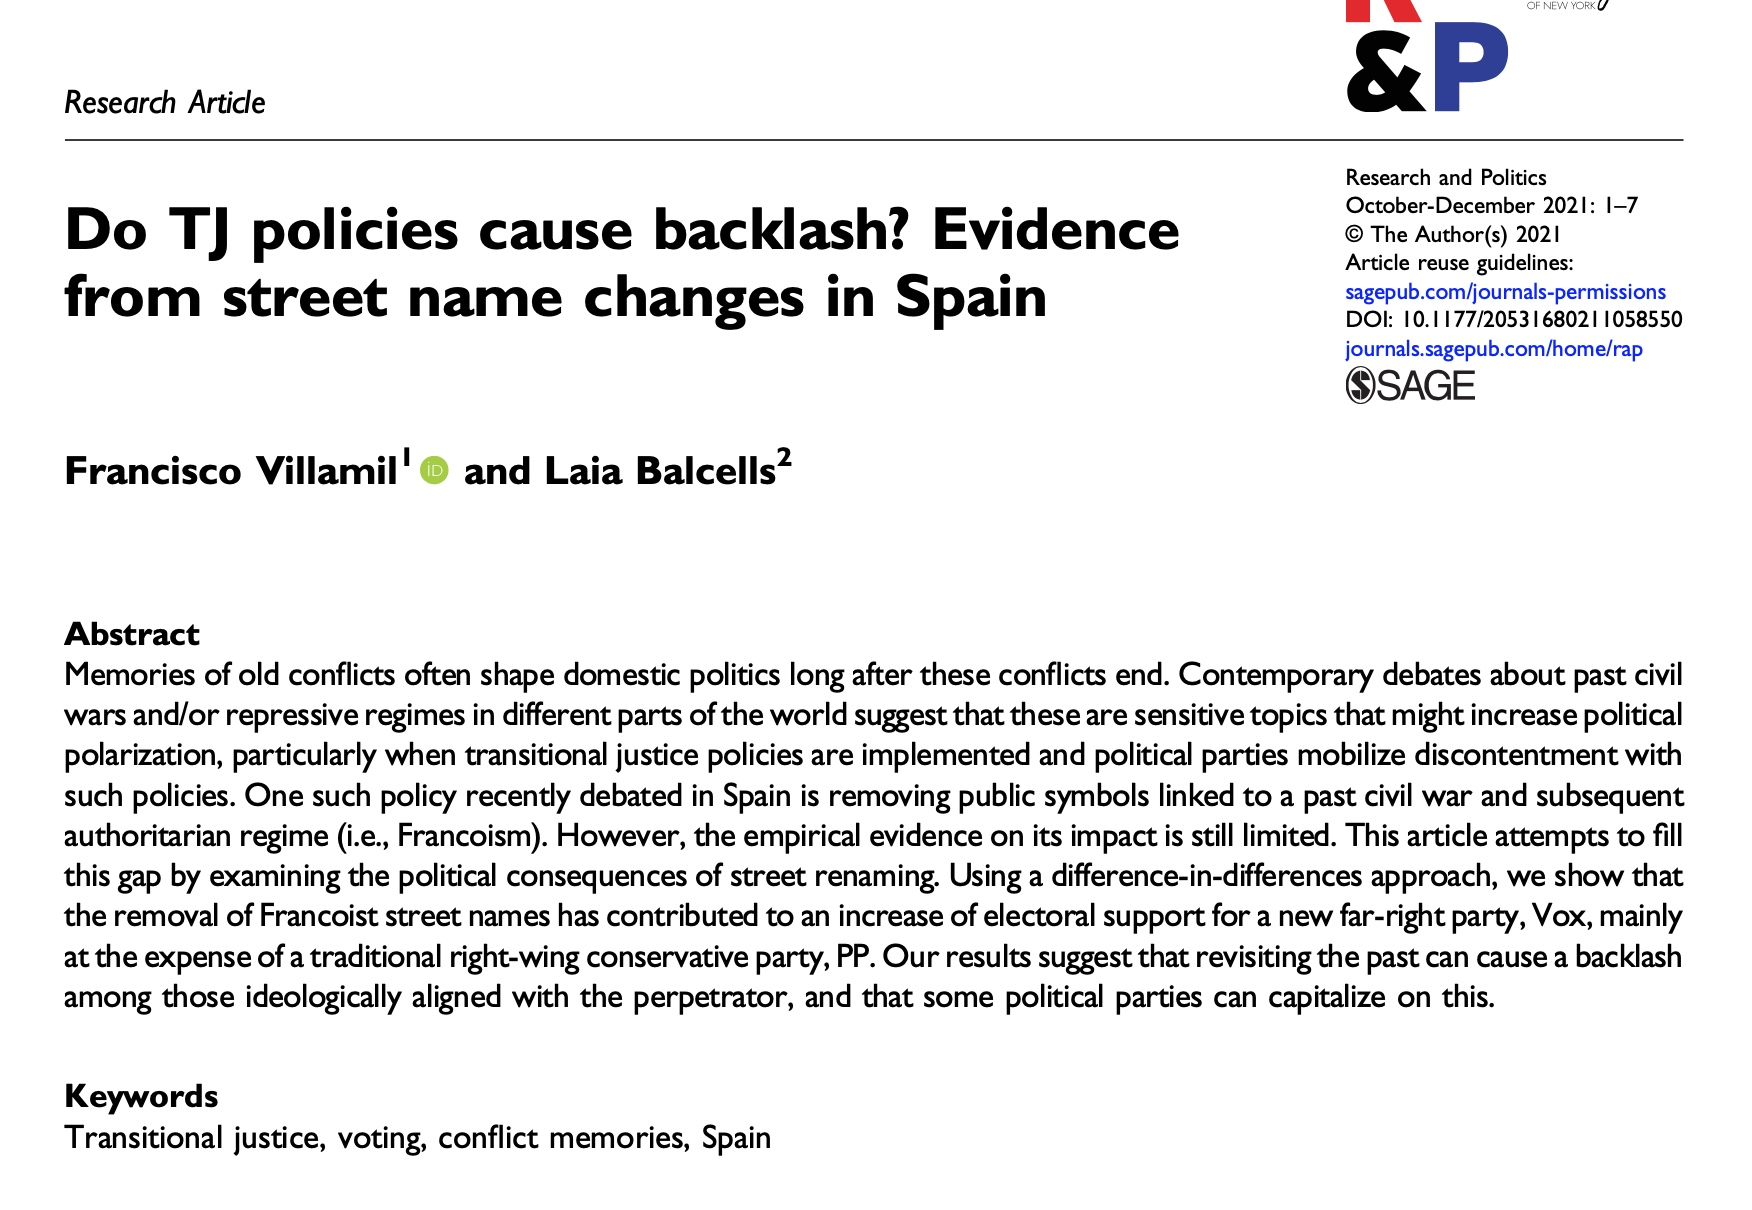
\includegraphics[width = \textwidth]{../img/villamilbalcells}

\end{frame}
% ----------------------------------------------------

\section{Re-cap and essay guidelines}

% ----------------------------------------------------
\begin{frame}
\frametitle{Re-cap and final essay}
\centering

\begin{itemize}
  \item \BGyellow{\textbf{Groups?}} Send me an email \textbf{before Oct 15th}
\end{itemize}

\end{frame}
% ----------------------------------------------------

% ----------------------------------------------------
\begin{frame}
\frametitle{Re-cap and final essay}
\centering

\begin{itemize}
  \item[1.] \BGyellow<1>{Problem/topic}
    \only<1>{\begin{itemize}
      \item unique to group, general issue
    \end{itemize}}
  \item[2.] \BGyellow<2>{Stories, arguments about mechanisms}
    \only<2>{\begin{itemize}
      \item testing an argument, testing 2 against each other
    \end{itemize}}
  \item[3.] \BGyellow<3>{Research question}
    \only<3>{\begin{itemize}
      \item operationalize the story you have in mind
    \end{itemize}}
  \item[4.] \BGyellow<4>{Proper theory, concepts and operationalization}
    \only<4>{\begin{itemize}
      \item develop a proper argument with view to empirical test
    \end{itemize}}
  \item[5.] \BGyellow<5>{Measurement, unit of analyses, data sources, etc}
    \only<5>{\begin{itemize}
      \item ideally think about more than one strategy
    \end{itemize}}
  \item[6.] \BGyellow<6>{Inference strategy}
    \only<6>{\begin{itemize}
      \item depends on previous steps: one per `arm' or multiple strategies
    \end{itemize}}
  \item[7.] \BGyellow<7>{Results \& interpretation}
    \only<7>{\begin{itemize}
      \item what do we really learn about the initial topic? next steps?
    \end{itemize}}
\end{itemize}

\only<8>{\begin{itemize}
  \item \textbf{General guideline:} maybe it's not realist you do it, but it needs to be feasible (data collection, etc)
\end{itemize}}

\end{frame}
% ----------------------------------------------------


% ----------------------------------------------------
\begin{frame}
\frametitle{Re-cap and final essay}
\centering

\begin{itemize}
  \item Logistics:
  \begin{itemize}
    \item 10-15 slots
    \item 10min presentation + 10min feedback
    \item If less groups, we can increase time
  \end{itemize}
  \item \textbf{Questions?}
\end{itemize}

\end{frame}
% ----------------------------------------------------

% ====================================================
\end{document}
